\subsection{Донгла Rockey: поиск неизвестного алгоритма используя только входные/выходные пары}

(Этот текст был впервые опубликован в августе 2012 в моем блоге: \url{http://blog.yurichev.com/node/71}.)

Некоторые смарткарты могут исполнять код на Java или .NET --- так можно спрятать какой-то важный алгоритм в чип,
который будет трудно взломать (декапсулировать).
Например, кто-то может шифровать/дешифровать файлы используя скрытый криптоалгоритм, что сделает
пиратство ПО близко к невозможному --- зашифрованный файл созданный на ПО с подключенной смарткартой
будет невозможно расшифровать на сломанном ПО.
(Впрочем, этому сопутствует масса неудобств.)

Это то, что называется \textit{черным ящиком}.

Некоторые донглы для защиты ПО также предлагают эти возможности.
Например, Rockey 4\footnote{\url{http://www.rockey.nl/en/rockey.html}}.

\begin{figure}[H]
\centering
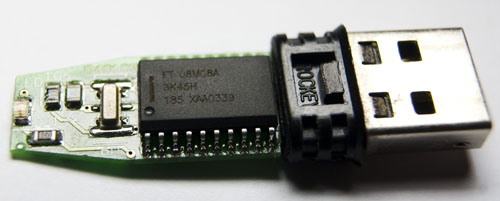
\includegraphics[scale=2]{pgm_synth/rockey_4.jpg}
\caption{Донгла Rockey 4}
\end{figure}

Это маленькая донгла подключаемая по USB. Содержит некоторую память для пользователя, а также память для пользовательских
алгоритмов.

Виртуальный (игрушечный) CPU для этих алгоритмов очень простой: он предлагает только 8 16-битных регистров
(хотя, только 4 из них можно выставлять и читать) и 8 операций
(сложение, вычитание, циклический сдвиг влево, умножение, ИЛИ, исключающее ИЛИ, И, отрицание).

Второй аргумент инструкции может быть константой (от 0 до 63) вместо регистра.

Каждый алгоритм определяется строкой вроде \\
\TT{A=A+B, B=C*13, D=D\^{}A, C=B*55, C=C\&A, D=D|A, A=A*9, A=A\&B}.

Памяти и стека нет, условных/безусловных переходов тоже, итд.

Всякий алгоритм, очевидно, не может иметь побочных эффектов, так что они, на самом деле, \textit{чистые функции},
и их результаты можно \textit{мемоизировать (memoization)}.

Кстати, как это было указано в документации к Rockey 4, первая и последняя инструкции не могут иметь констант.
Может быть это потому что эти поля используются для какой-то внутренней информации:
начало и конец каждого алгоритма должны же как-то маркироваться.

Можно ли узнать внутренний алгоритм, который невозможно прочитать, только наблюдая входной/выходной траффик донглы?
Общая точка зрения на это ``нет''. Но мы всё же попробуем.

Так как моя цель была не в том, что бы взломать ПО защищенное Rockey,
мне было только интересно узнать пределы (какие алгоритмы мы можем найти),
так что я немного всё упростил: мы будем работать только с четырьмя 16-битными регистрами,
и здесь будут только 6 операций (сложение, вычитание, умножение, ИЛИ, исключающее ИЛИ, И).

В начале, подсчитаем, как много информации будет использовано в случае брутфорса.

Всего возможно 384 инструкции вида \TT{reg=reg,op,reg} для 4-х регистров и 6-и операций,
а также 6144 инструкций вида \TT{reg=reg,op,constant}.
Помните, что каждая константа ограничена максимальным значением в 63? Это нам немного поможет.

Так что здесь всего 6528 возможных инструкций.
Это означает, что здесь $\approx 1.1 \cdot 10^{19}$ возможных алгоритмов из 5-и инструкций.
Это многовато.

Как можно выразить каждую инструкцию как систему уравнений?
Пока я вспоминал школьную математику, я написал это:

\begin{lstlisting}
Функция one\_step()=

# Каждая Bx это целочисленное, может быть только 0 или 1.

# Только одна из B1..B4 и B5..B9 может быть выставлена
reg1=B1*A + B2*B + B3*C + B4*D
reg_or_constant2=B5*A + B6*B + B7*C + B8*D + B9*константа
reg1 не должен быть равен reg_or_constant2

# Только одна из B10..B15 может быть выставлена
result=result+B10*(reg1*reg2)
result=result+B11*(reg1^reg2)
result=result+B12*(reg1+reg2)
result=result+B13*(reg1-reg2)
result=result+B14*(reg1|reg2)
result=result+B15*(reg1&reg2)

B16 - истинна, если регистр не обновляется в этой части
B17 - истинна если регистр обновляется в этой части
(B16 не может быть равно B17)
A=B16*A + B17*result
B=B18*A + B19*result
C=B20*A + B21*result
D=B22*A + B23*result
\end{lstlisting}

Так можно выразить каждую инструкцию в алгоритме.

Алгоритм из пяти инструкций можно выразить так:\\
\TT{one\_step (one\_step (one\_step (one\_step (one\_step (input\_registers)))))}.

Добавим пять известных входных/выходных пар, и получим систему уравнений вроде:

\begin{lstlisting}
one_step (one_step (one_step (one_step (one_step (input_1)))))==output_1
one_step (one_step (one_step (one_step (one_step (input_2)))))==output_2
one_step (one_step (one_step (one_step (one_step (input_3)))))==output_3
one_step (one_step (one_step (one_step (one_step (input_4)))))==output_4
.. итд
\end{lstlisting}

Теперь вопрос это, как найти $5 \cdot 23$ булевых значений, удовлетворяющих известные входные/выходные пары.

Я написал маленькую утилиту для подачи случайных значений в алгоритм в Rockey 4, и он выдает результаты в виде:

\begin{lstlisting}
RY_CALCULATE1: (input) p1=30760 p2=18484 p3=41200 p4=61741 (output) p1=49244 p2=11312 p3=27587 p4=12657
RY_CALCULATE1: (input) p1=51139 p2=7852 p3=53038 p4=49378 (output) p1=58991 p2=34134 p3=40662 p4=9869
RY_CALCULATE1: (input) p1=60086 p2=52001 p3=13352 p4=45313 (output) p1=46551 p2=42504 p3=61472 p4=1238
RY_CALCULATE1: (input) p1=48318 p2=6531 p3=51997 p4=30907 (output) p1=54849 p2=20601 p3=31271 p4=44794
\end{lstlisting}

p1/p2/p3/p4 это просто другие названия регистров A/B/C/D.

Теперь начнем с Z3. Нам нужно выразить игрушечный CPU Rockey 4 в терминах Z3Py (Z3 Python \ac{API}).

Можно сказать, мой Питоновский скрипт разделен на две части:

\begin{itemize}
\item определение констрайнтов (вроде, \textit{output\_1 должен быть $n$ для input\_1=m},
\textit{константа не может быть больше 63}, итд); 

\item ф-ции, конструирующие систему уравнение.
\end{itemize}

Этот фрагмент кода определяет некоторую \textit{структуру} состоящую из 4 16-битных переменных,
каждая представляет собой регистр в нашем игрушечном \ac{CPU}:

\begin{lstlisting}
Registers_State=Datatype ('Registers_State')
Registers_State.declare('cons', ('A', BitVecSort(16)), ('B', BitVecSort(16)), ('C', BitVecSort(16)), ('D', BitVecSort(16)))
Registers_State=Registers_State.create()
\end{lstlisting}

Эти перечисления определяют два новых типа (или \textit{sort}-а в терминологии Z3):

\begin{lstlisting}
Operation, (OP_MULT, OP_MINUS, OP_PLUS, OP_XOR, OP_OR, OP_AND) = EnumSort('Operation', ('OP_MULT', 'OP_MINUS', 'OP_PLUS', 'OP_XOR', 'OP_OR', 'OP_AND'))

Register, (A, B, C, D) = EnumSort('Register', ('A', 'B', 'C', 'D'))
\end{lstlisting}

Эта часть очень важная, она определяет все переменные в нашей системе уравнений.
\TT{op\_step} это тип операции в инструкции.
\TT{reg\_or\_constant} это селектор между регистром и константой во втором аргументе ---
\textit{False}, если это регистр и \textit{True}, если это константа.
\TT{reg\_step} это регистр-приемник в этой инструкции.
\TT{reg1\_step} и \TT{reg2\_step} это просто регистры на arg1 and arg2. 
\TT{constant\_step} это константа (в случае, если она используется в регистре вместо arg2).

\begin{lstlisting}
op_step=[Const('op_step%s' % i, Operation) for i in range(STEPS)]
reg_or_constant_step=[Bool('reg_or_constant_step%s' % i) for i in range(STEPS)]
reg_step=[Const('reg_step%s' % i, Register) for i in range(STEPS)]
reg1_step=[Const('reg1_step%s' % i, Register) for i in range(STEPS)]
reg2_step=[Const('reg2_step%s' % i, Register) for i in range(STEPS)]
constant_step = [BitVec('constant_step%s' % i, 16) for i in range(STEPS)]
\end{lstlisting}

Добавление констрайнтов это просто. Помните, я писал что каждая константа не может быть больше 63?

\begin{lstlisting}
# согласно документации к донгле Rockey 4, arg2 в первой и второй инструкции не могут быть константой
s.add (reg_or_constant_step[0]==False)
s.add (reg_or_constant_step[STEPS-1]==False)

...

for x in range(STEPS):
   s.add (constant_step[x]>=0, constant_step[x]<=63)
\end{lstlisting}

Известные входные/выходные значения также добавляются как констрайнты.

Посмотрим, как сконструировать нашу систему уравнений:

\begin{lstlisting}
# Register, Registers_State -> int
def register_selector (register, input_registers):
    return If(register==A, Registers_State.A(input_registers),
           If(register==B, Registers_State.B(input_registers), 
           If(register==C, Registers_State.C(input_registers), 
           If(register==D, Registers_State.D(input_registers), 
                           0)))) # default
\end{lstlisting}

Это ф-ция возвращающая значение соответствующего регистра из \textit{структуры}.
Нужно сказать, что этот код не исполняется.
\TT{If()} это ф-ция Z3Py. 
Этот код только объявляет ф-цию, которая будет использована в другой.
Объявление выражений немного напоминает ЯП LISP.

Вот еще одна ф-ция, где используется \TT{register\_selector()}:

\begin{lstlisting}
# Bool, Register, Registers_State, int -> int
def register_or_constant_selector (register_or_constant, register, input_registers, constant): 
    return If(register_or_constant==False, register_selector(register, input_registers), constant)
\end{lstlisting}

Этот код здесь тоже никогда не будет исполнен.
Он только конструирует одну маленькую часть очень большого выражения.
Но ради упрощения понимания, можно думать, что все эти ф-ции будут вызываться во время брутфорса, много раз,
на самой большой возможной скорости.

\begin{lstlisting}
# Operation, Bool, Register, Register, Int, Registers_State -> int
def one_op (op, register_or_constant, reg1, reg2, constant, input_registers):
    arg1=register_selector(reg1, input_registers)
    arg2=register_or_constant_selector (register_or_constant, reg2, input_registers, constant)
    return If(op==OP_MULT,   arg1*arg2,
           If(op==OP_MINUS,  arg1-arg2,
           If(op==OP_PLUS,   arg1+arg2, 
           If(op==OP_XOR,    arg1^arg2, 
           If(op==OP_OR,     arg1|arg2, 
           If(op==OP_AND,    arg1&arg2, 
                          0)))))) # default
\end{lstlisting}

Вот выражение описывающее каждую инструкцию.
Регистру-приемнику здесь будет присвоено \TT{new\_val},
в то время как значения остальных регистров копируются из входного состояния входных регистров:

% FIXME: at_this_step!

\begin{lstlisting}
# Bool, Register, Operation, Register, Register, Int, Registers_State -> Registers_State
def one_step (register_or_constant, register_assigned_in_this_step, op, reg1, reg2, constant, input_registers):
    new_val=one_op(op, register_or_constant, reg1, reg2, constant, input_registers)
    return If (register_assigned_in_this_step==A, Registers_State.cons (new_val,
                                                                        Registers_State.B(input_registers), 
                                                                        Registers_State.C(input_registers), 
                                                                        Registers_State.D(input_registers)),
           If (register_assigned_in_this_step==B, Registers_State.cons (Registers_State.A(input_registers), 
                                                                        new_val,
                                                                        Registers_State.C(input_registers),
                                                                        Registers_State.D(input_registers)), 
           If (register_assigned_in_this_step==C, Registers_State.cons (Registers_State.A(input_registers), 
                                                                        Registers_State.B(input_registers), 
                                                                        new_val,
                                                                        Registers_State.D(input_registers)), 
           If (register_assigned_in_this_step==D, Registers_State.cons (Registers_State.A(input_registers), 
                                                                        Registers_State.B(input_registers), 
                                                                        Registers_State.C(input_registers), 
                                                                        new_val),
                                                  Registers_State.cons(0,0,0,0))))) # default
\end{lstlisting}

Это последняя ф-ция, описывающая всю программу из $n$ шагов:

\begin{lstlisting}
def program(input_registers, STEPS):
    cur_input=input_registers
    for x in range(STEPS):
        cur_input=one_step (reg_or_constant_step[x], reg_step[x], op_step[x], reg1_step[x], reg2_step[x], constant_step[x], cur_input)
    return cur_input
\end{lstlisting}

И снова, ради простоты, можно сказать, что теперь Z3 будет пробовать каждые возможные
регистры/операции/константы на этом выражении, в поиске такой комбинации, которая удовлетворит все входные/выходные пары.
Звучит абсурдно, но это близко к реальности.
SAT/SMT-солверы действительно пробуют их все.
Но их сложность в том, что бы отсекать поисковое дерево как можно раньше, так что вся эта штука будет работать
какое-то приемлимое время.
И это самая трудная проблема для солверов.

Теперь начнем с очень простого алгоритма из 3 шагов: \TT{B=A\^{}D, C=D*D, D=A*C}.
Нужно отметить: регистр \TT{A} остается неизменным.
Я запрограммировал донглу Rockey 4 с этим алгоритмом, и вот результаты:

\begin{lstlisting}
RY_CALCULATE1: (input) p1=8803 p2=59946 p3=36002 p4=44743 (output) p1=8803 p2=36004 p3=7857 p4=24691
RY_CALCULATE1: (input) p1=5814 p2=55512 p3=52155 p4=55813 (output) p1=5814 p2=52403 p3=33817 p4=4038
RY_CALCULATE1: (input) p1=25206 p2=2097 p3=55906 p4=22705 (output) p1=25206 p2=15047 p3=10849 p4=43702
RY_CALCULATE1: (input) p1=10044 p2=14647 p3=27923 p4=7325 (output) p1=10044 p2=15265 p3=47177 p4=20508
RY_CALCULATE1: (input) p1=15267 p2=2690 p3=47355 p4=56073 (output) p1=15267 p2=57514 p3=26193 p4=53395
\end{lstlisting}

Заняло около секунды и только 5 вышеуказанных пар, чтобы найти алгоритм
(на моем четырехядерном Xeon E3-1220 3.1GHz, впрочем, солвер Z3 работает только в одном треде):

\begin{lstlisting}
B = A ^ D
C = D * D
D = C * A
\end{lstlisting}

Теперь последняя инструкция: регистры \TT{C} и \TT{A} поменены местами, если сравнить с версией, которую я написал вручную.
Конечно, эта инструкция работает так же, ведь умножение это коммутативная операция.

Теперь попробуем найти программу из 4-х шагов, удовлетворяющую этим значениям, и мой скрипт предложил вот это:

\begin{lstlisting}
B = A ^ D
C = D * D
D = A * C
A = A | A
\end{lstlisting}

\dots и это даже смешно, в некотором смысле, потому что последняя инструкция ничего не делает со значением в регистре \TT{A},
это как \ac{NOP} --- но все же, алгоритм корректен для всех этих данных значений.

Вот еще один алгоритм из 5-и шагов: \TT{B=B\^{}D, C=A*22, A=B*19, A=A\&42, D=B\&C} и значения:

\begin{lstlisting}
RY_CALCULATE1: (input) p1=61876 p2=28737 p3=28636 p4=50362 (output) p1=32 p2=46331 p3=50552 p4=33912
RY_CALCULATE1: (input) p1=46843 p2=43355 p3=39078 p4=24552 (output) p1=8 p2=63155 p3=47506 p4=45202
RY_CALCULATE1: (input) p1=22425 p2=51432 p3=40836 p4=14260 (output) p1=0 p2=65372 p3=34598 p4=34564
RY_CALCULATE1: (input) p1=44214 p2=45766 p3=19778 p4=59924 (output) p1=2 p2=22738 p3=55204 p4=20608
RY_CALCULATE1: (input) p1=27348 p2=49060 p3=31736 p4=59576 (output) p1=0 p2=22300 p3=11832 p4=1560
\end{lstlisting}

Заняло 37 секунд, и мы получаем:

\begin{lstlisting}
B = D ^ B
C = A * 22
A = B * 19
A = A & 42
D = C & B
\end{lstlisting}

\TT{A=A\&42} было найдено корректно (посмотрите на пять выходов p1 (присвоенных регистру \TT{A}): 32,8,0,2,0)

Алгоритм из 6-и шагов \TT{A=A+B, B=C*13, D=D\^{}A, C=C\&A, D=D|B, A=A\&B} и значения:

\begin{lstlisting}
RY_CALCULATE1: (input) p1=4110 p2=35411 p3=54308 p4=47077 (output) p1=32832 p2=50644 p3=36896 p4=60884
RY_CALCULATE1: (input) p1=12038 p2=7312 p3=39626 p4=47017 (output) p1=18434 p2=56386 p3=2690 p4=64639
RY_CALCULATE1: (input) p1=48763 p2=27663 p3=12485 p4=20563 (output) p1=10752 p2=31233 p3=8320 p4=31449
RY_CALCULATE1: (input) p1=33174 p2=38937 p3=54005 p4=38871 (output) p1=4129 p2=46705 p3=4261 p4=48761
RY_CALCULATE1: (input) p1=46587 p2=36275 p3=6090 p4=63976 (output) p1=258 p2=13634 p3=906 p4=48966
\end{lstlisting}

90 секунд и получаем:

\begin{lstlisting}
A = A + B
B = C * 13
D = D ^ A
D = B | D
C = C & A
A = B & A
\end{lstlisting}

Хотя это и было просто.
Некоторые алгоритмы из 6-и шагов не удается найти, например:\\
\TT{A=A\^{}B, A=A*9, A=A\^{}C, A=A*19, A=A\^{}D, A=A\&B}.
Солвер работал слишком долго (вплоть до нескольких часов), так что я даже и не знаю, возможно ли его вообще найти.

\subsubsection{Вывод}

На самом деле, это простое упраженние в синтезе программ.

Некоторые короткие алгоритмы для крохотных \ac{CPU} действительно возможно найти используя небольшой набор данных.
Конечно, более сложные алгоритмы найти невозможно,
но этот метод однозначно нельзя игнорировать.

\subsubsection{Файлы}

Программатор и дампер донглы Rockey 4, документация Rockey 4, скрипт Z3Py для поиска алгоритмов, входные/выходные пары:
\url{https://github.com/dennis714/SAT_SMT_article/tree/master/pgm_synth/rockey_files}.

\subsubsection{Дальнейшая работа}

Возможно, конструирование LISP-подобных S-выражений может быть лучше, чем программирование игрушечного CPU.

Также, можно начинать с м\'{е}ньших констант и постепенно переходить к б\'{о}льшим.
Это немного напоминает, как постепенно удлиняется длина пароля во время брутфорса паролей.

